\documentclass[../document.tex]{subfiles}
\begin{document}
\chapter{Methodology}
We develop a framework to learn traversability directly on ground patches for any robot using purely simulated data. The core idea, originally proposed by Chavez-Garcia et al. \cite{omar2018traversability}, is simple, we let a robot travel into a simulator on different synthetic terrain, we store its interactions to later crop a region of ground, a patch, around each traveled position and directly train a neural network on them to predict traversability. Figure \ref{fig : pipeline} shows the proposed framework.
\begin{figure}[H]
    \centering
        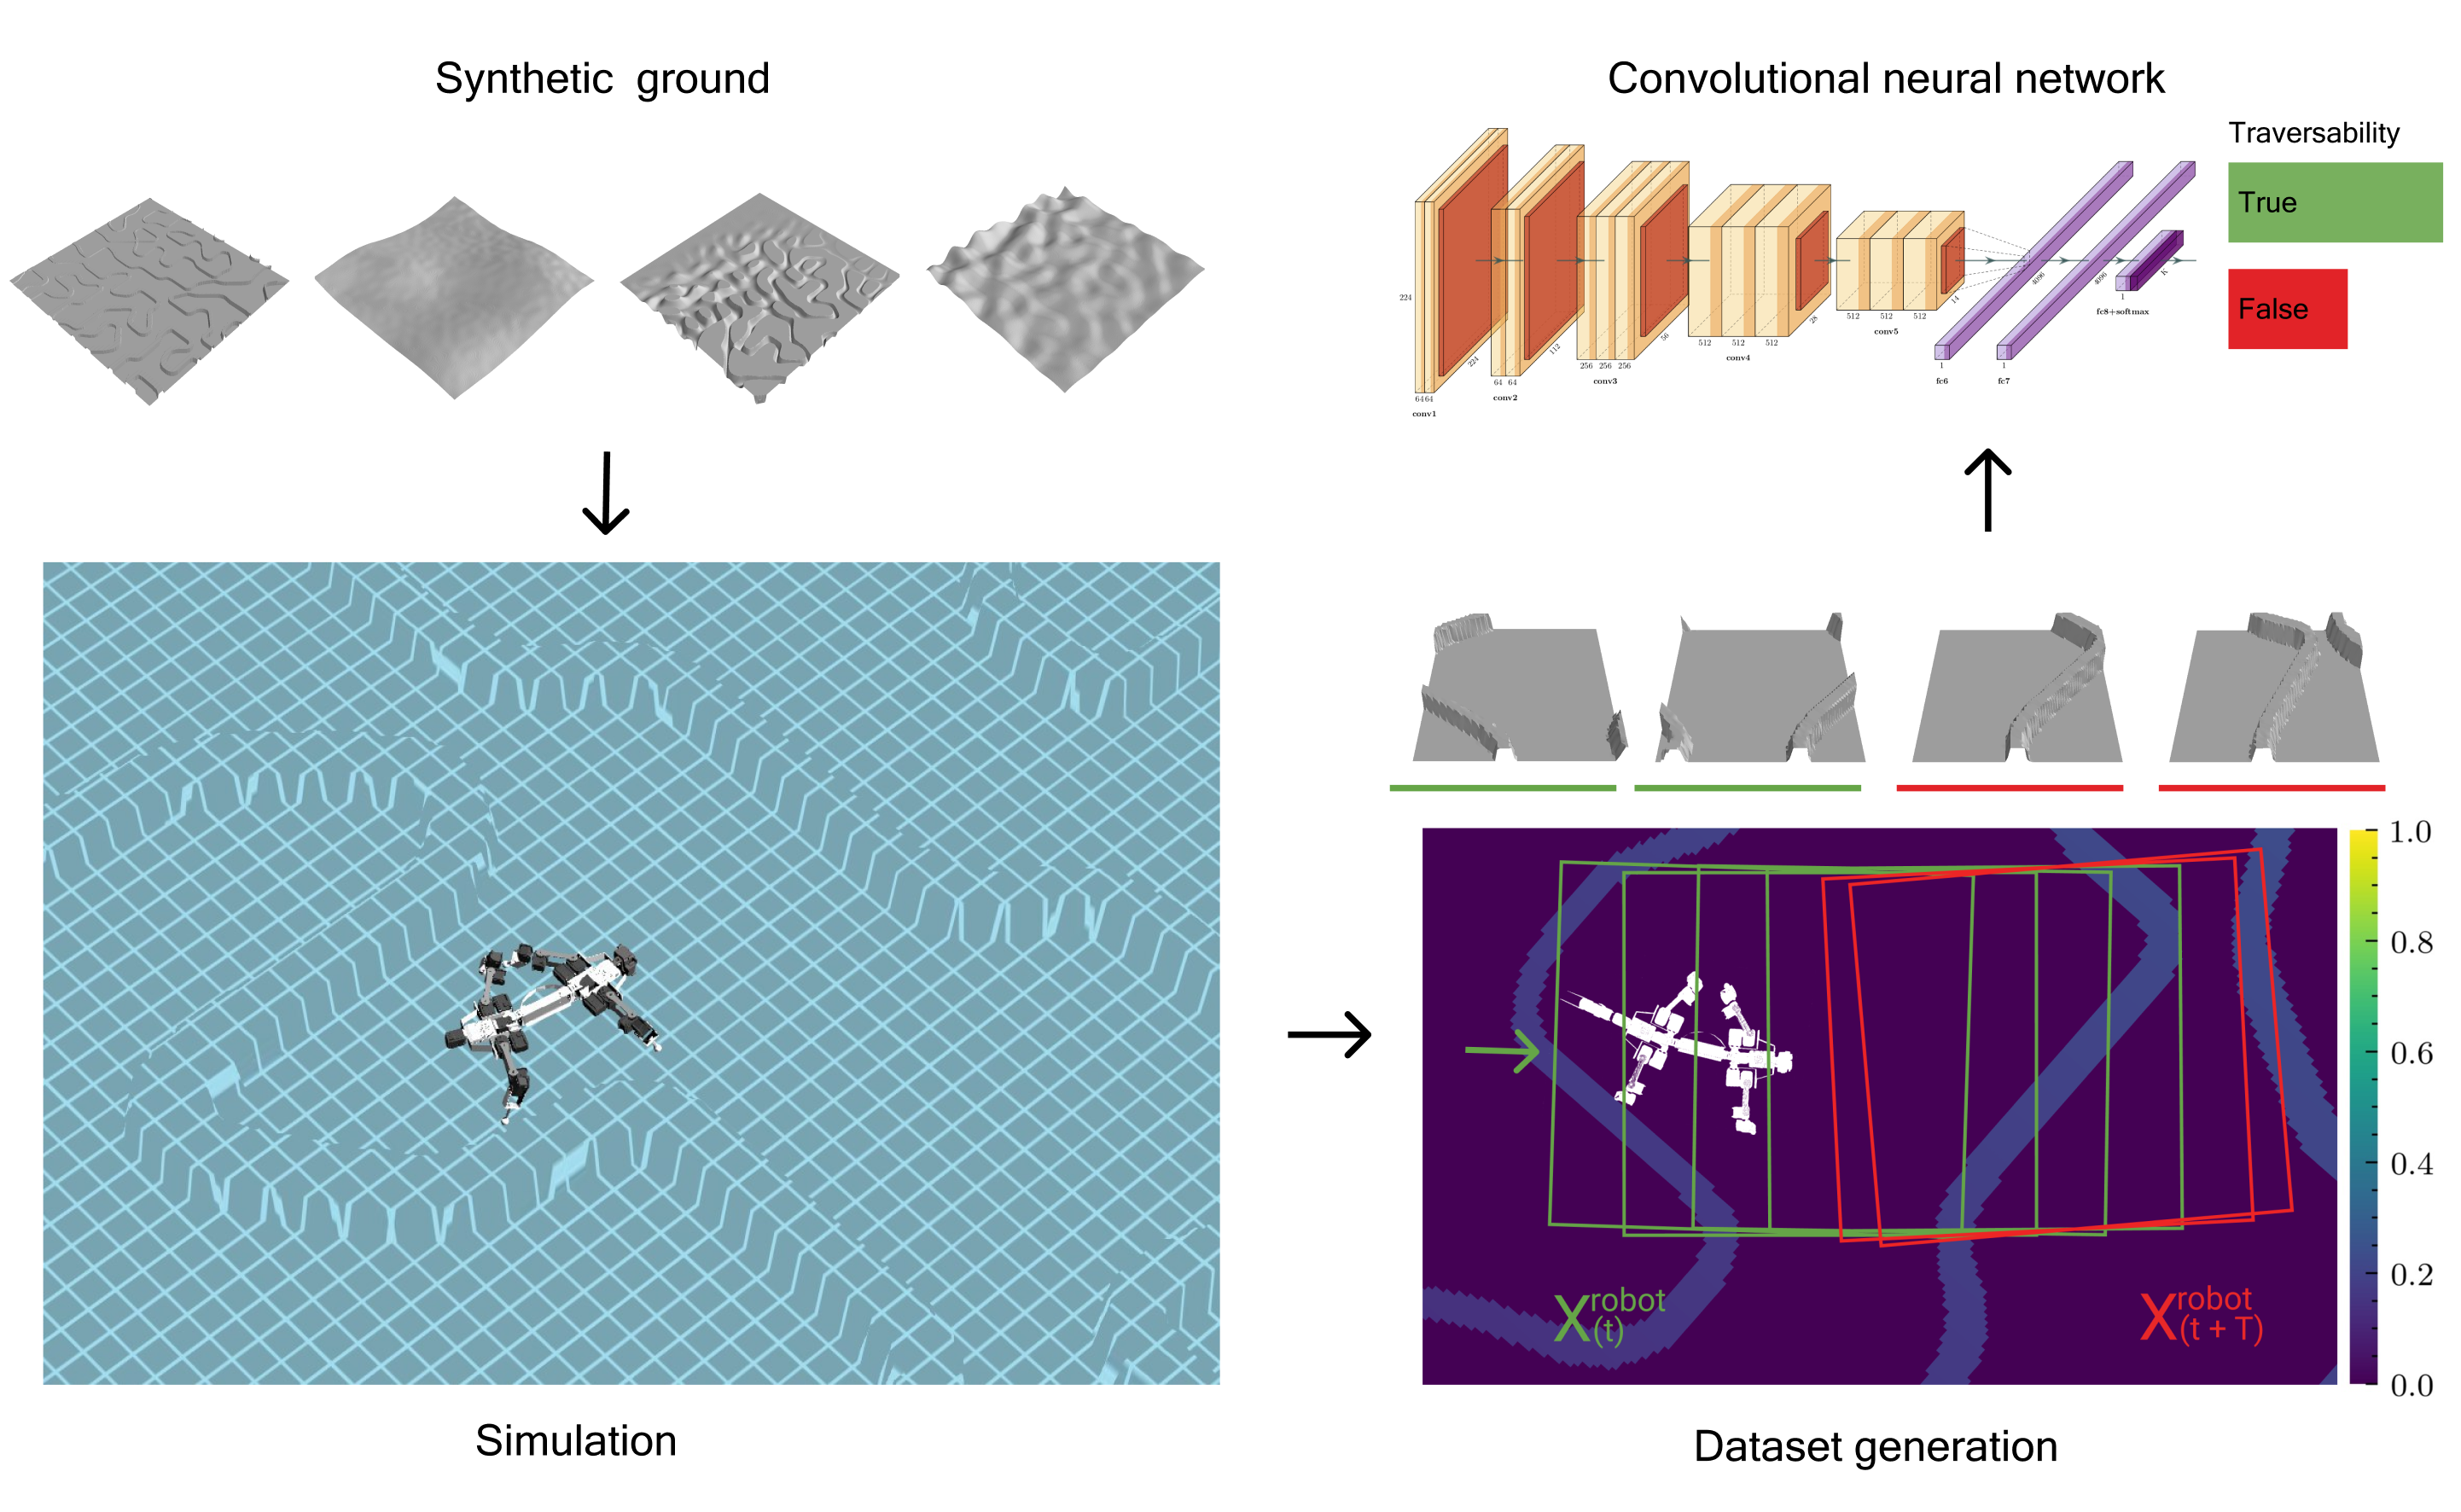
\includegraphics[width=\textwidth]{../img/method.png}
    \caption{The proposed traversability framework's main blocks in couter-clockwise order. First we generated meaningful synthetic ground, then we let the robot spawn and walk on them in simulated enviroment while storing its interactions. Later, we crop a region of ground, a patch, for each simulation trajectory around the robot according to its locomotion. We label those images using a defined treshold and fit a deep convolutional neural network to predict traversability. }
    \label{fig : pipeline}
    \end{figure}
Collecting data trought simulation data has three main advantages: variety, cost, and speed. With simulations, we can easily increase the number of data samples by just include more maps, while doing the same with a real robot requires to first identify the suitable ground and then travel to it. Clearly, this also decreases the time required to collect the robot's interaction with the ground. The time could be additional decreased by running different simulations in parallel avoiding physical manufacture or purchase additional robots. 
Moreover, we are not limited by real constraint and therefore the robot can interact with a multitude of different grounds. For instance, to collect real-world data the robot must be physically transported to different locations, on the other hand, with simulations we can immediately load a new map.
To create a quality dataset, we must first generate a series of various surfaces and ensure their diversity. Intuitively, those maps should be small enough to allow fast interactions with their features but big enough to include variety. With modern ground generation techniques, it is fairly straightforward to generate a rich array of terrains with different characteristics such us bumps, ramps, slopes in different levels and sizes. These images are stored as gray images where the brightness represent the height. The following figure shows an small collection of synthetic terrains with different features.
\begin{figure}[H]
    \centering
    \begin{subfigure}[b]{0.24\textwidth}
        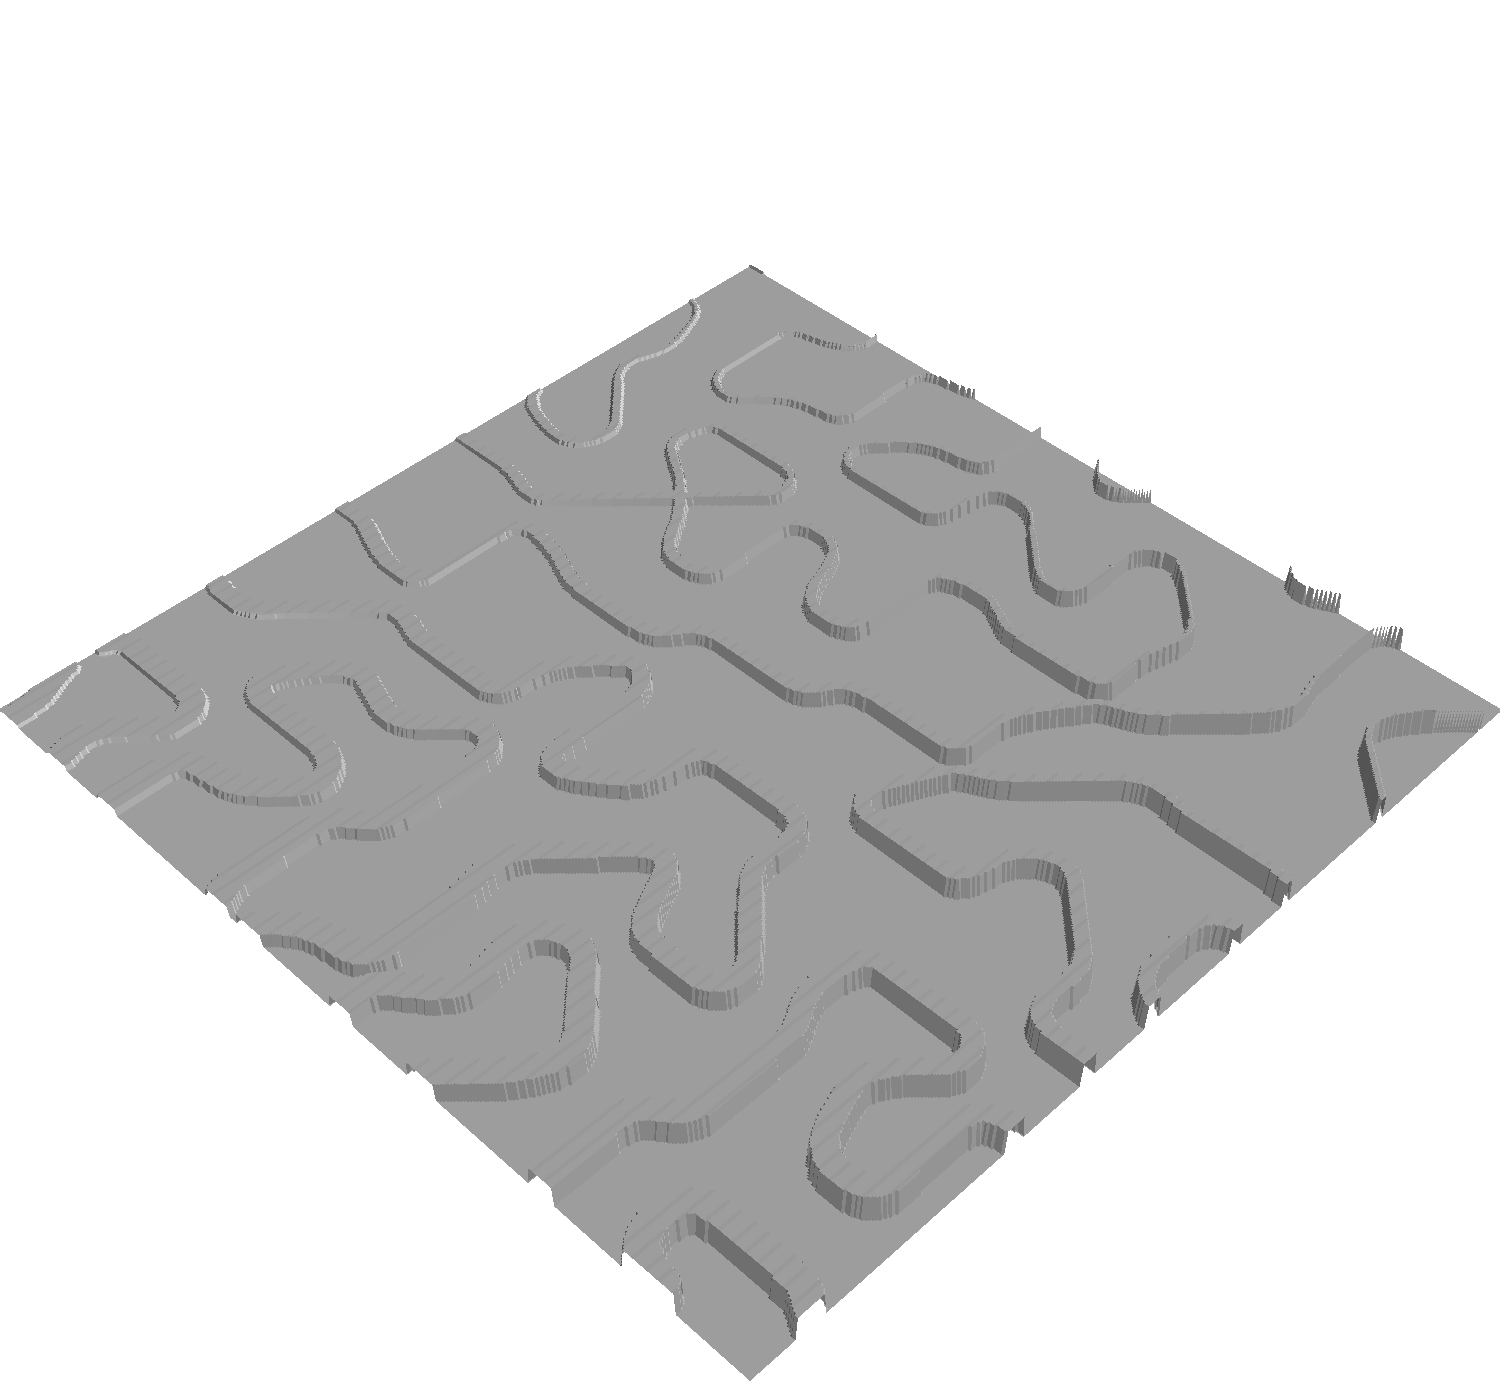
\includegraphics[width=\linewidth]{../img/hm3d/bars1.png}
        \caption{Walls.}
    \end{subfigure}
    \begin{subfigure}[b]{0.24\textwidth}
        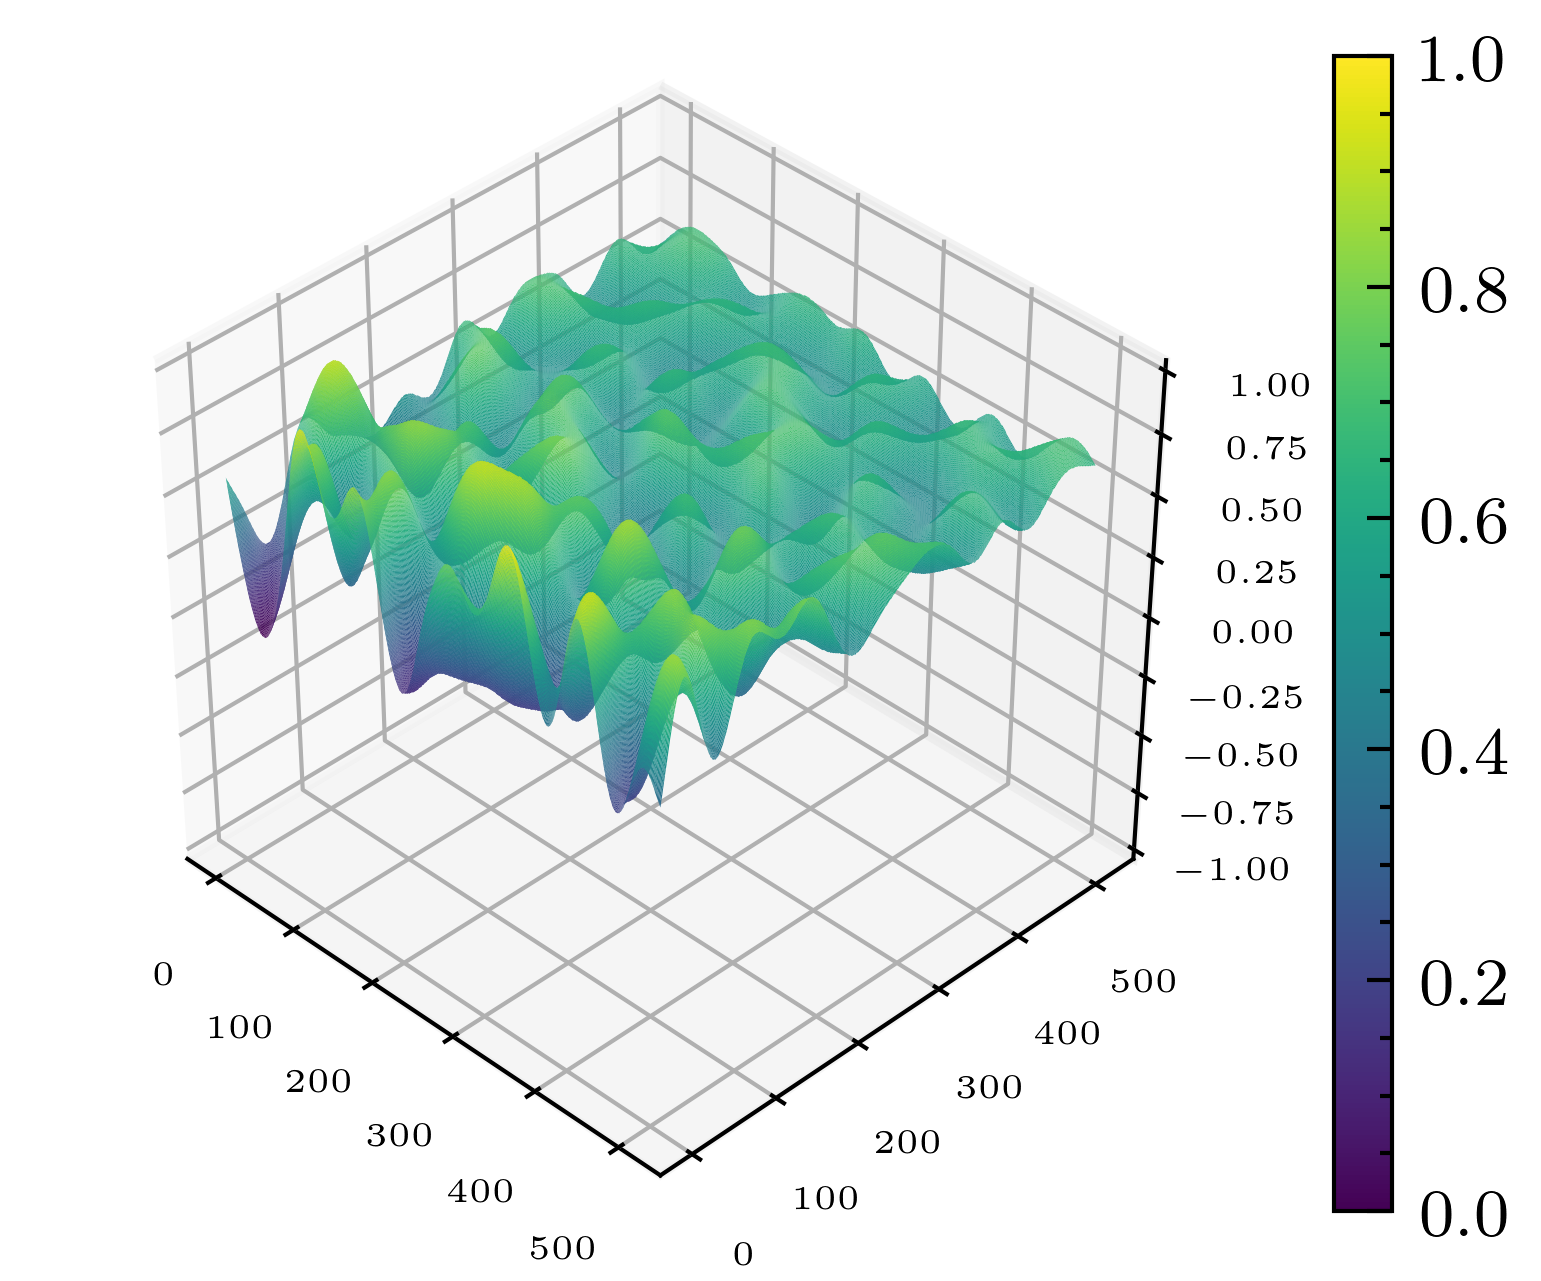
\includegraphics[width=\linewidth]{../img/hm3d/bumps2.png}
        \caption{Bumps.}
 \end{subfigure}  
    \begin{subfigure}[b]{0.24\textwidth}
        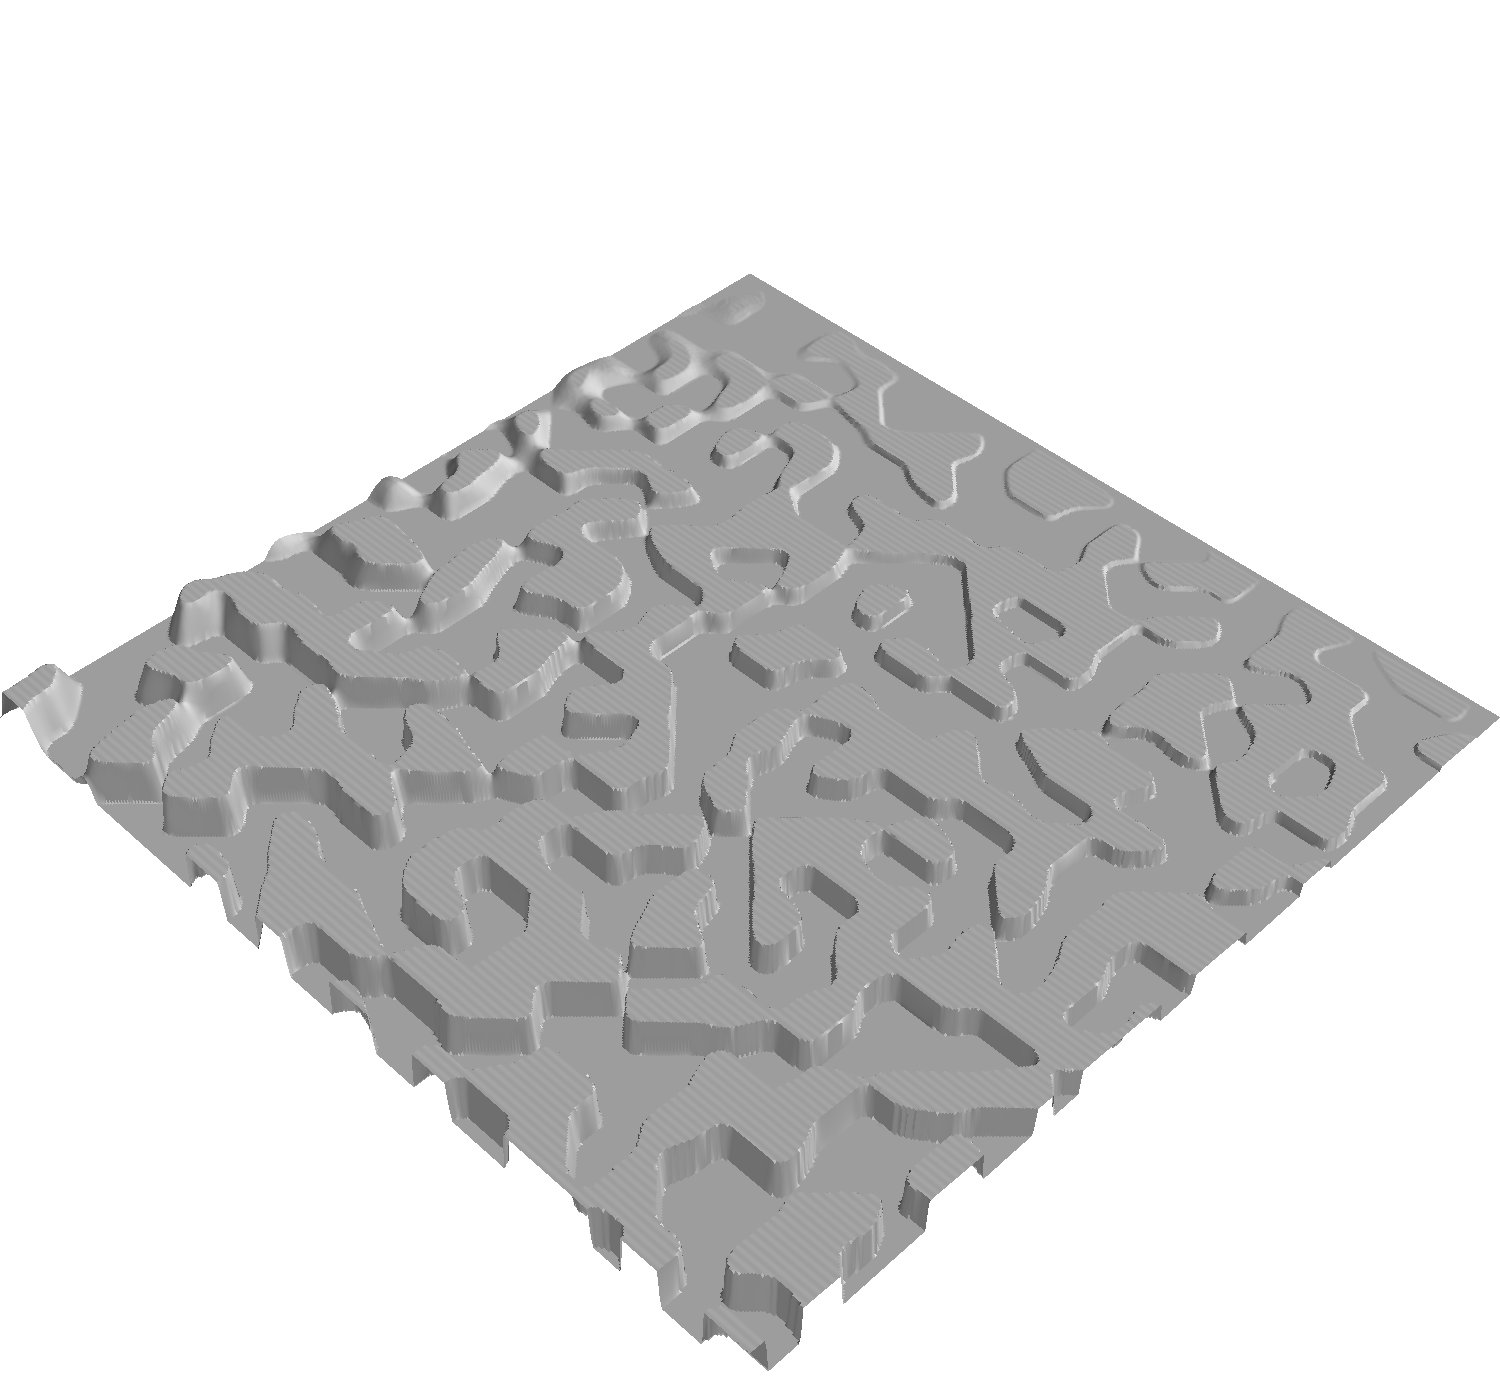
\includegraphics[width=\linewidth]{../img/hm3d/steps1.png}
        \caption{Steps.}
 \end{subfigure}  
    \begin{subfigure}[b]{0.24\textwidth}
        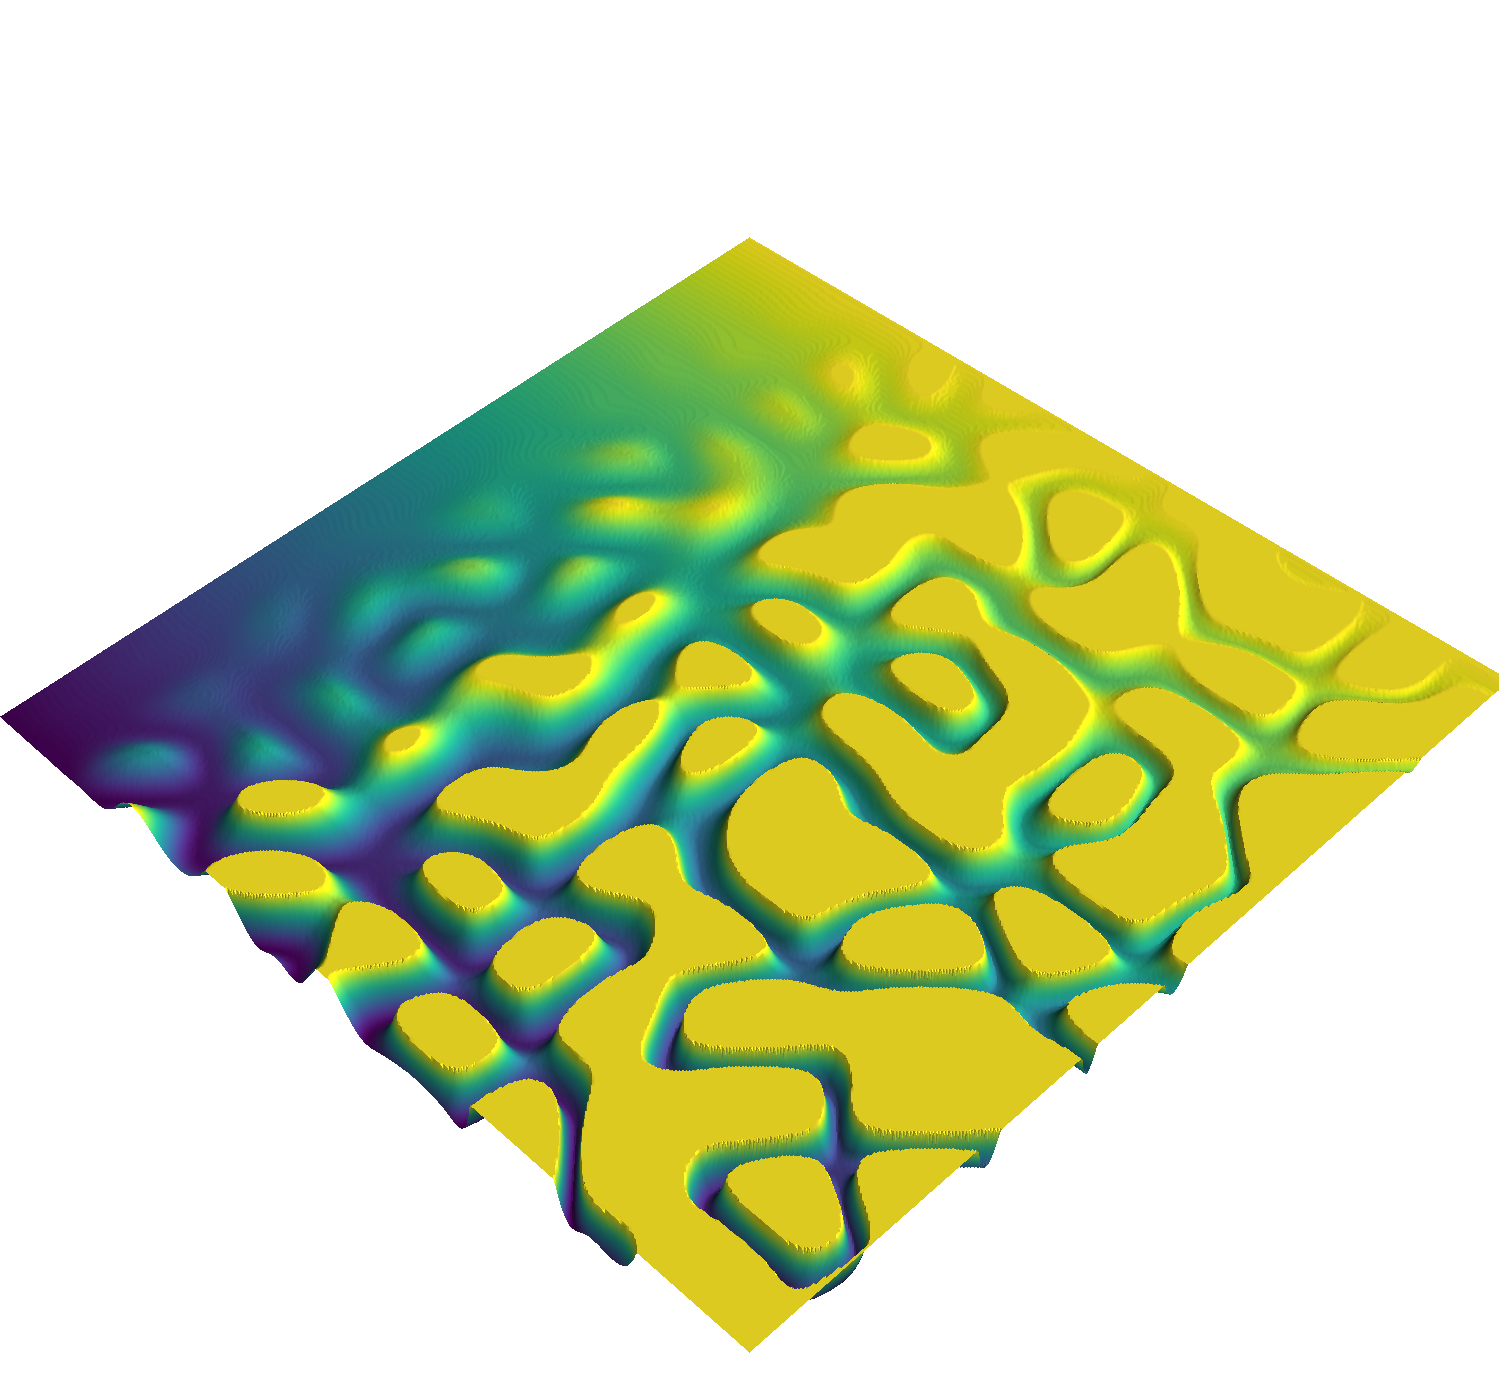
\includegraphics[width=\linewidth]{../img/hm3d/rails3.png}
        \caption{Rails.}
    \end{subfigure}  
\caption{Some artificially generated terrains, $10\times 10$m, with one specific feature each. }   
\end{figure}
The maps can be loaded into a simulator to let the robot interact with them. To ensure a correct exploration of each terrain, it is better to randomly spawn the robot multiple times on the same map and let it walk for a fixed amount of time. The robot position is tracked and stored during simulation in order to extract a small portion of ground, patches, around each of its trajectory's position. In practice, the patches are cropped from the original image using a specific size based on the robot's footprint and its locomotion. Each resulting image is label using a minimum advancement defined for the robot. We tested our framework on a legged crocodile-like robot called \emph{Krock}. This robot's has a very special locomotion that allows it to overcome different obstacles making the estimantion not trivial.  Figure \ref{patch-extraction} helps visualize the procedure.
\begin{figure}[H]
    \centering
    \begin{subfigure}[b]{0.66\textwidth}
    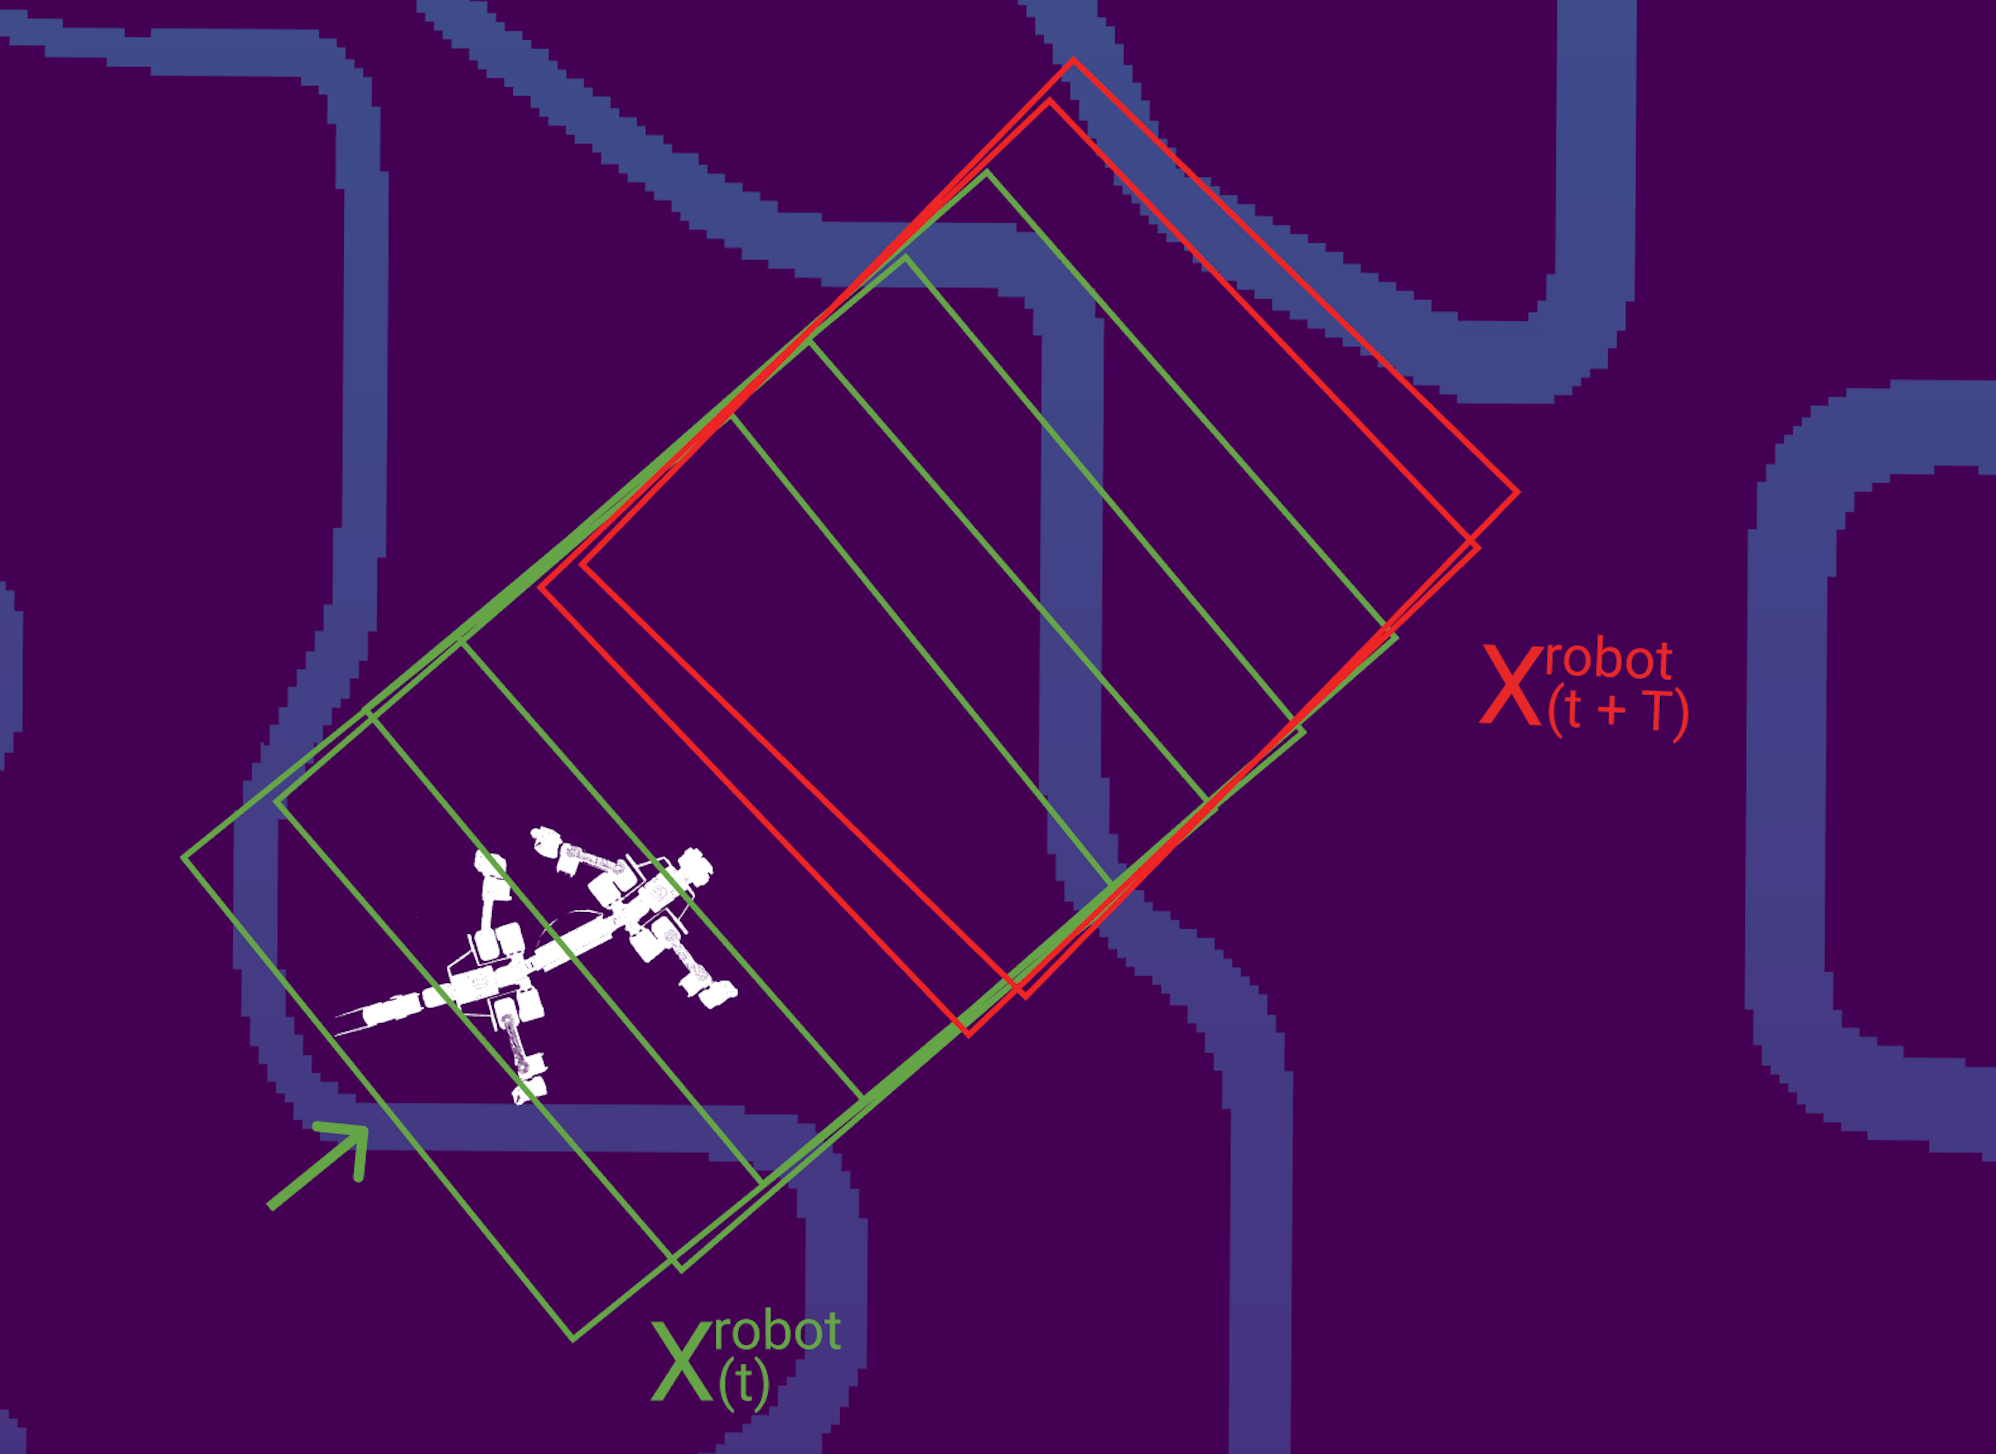
\includegraphics[width=\textwidth]{../img/krock-bars-correct-small.png}
    \caption{Robot's trajectory.}
\end{subfigure}
\begin{subfigure}[b]{1\textwidth}
    \begin{subfigure}[b]{0.19\textwidth}
    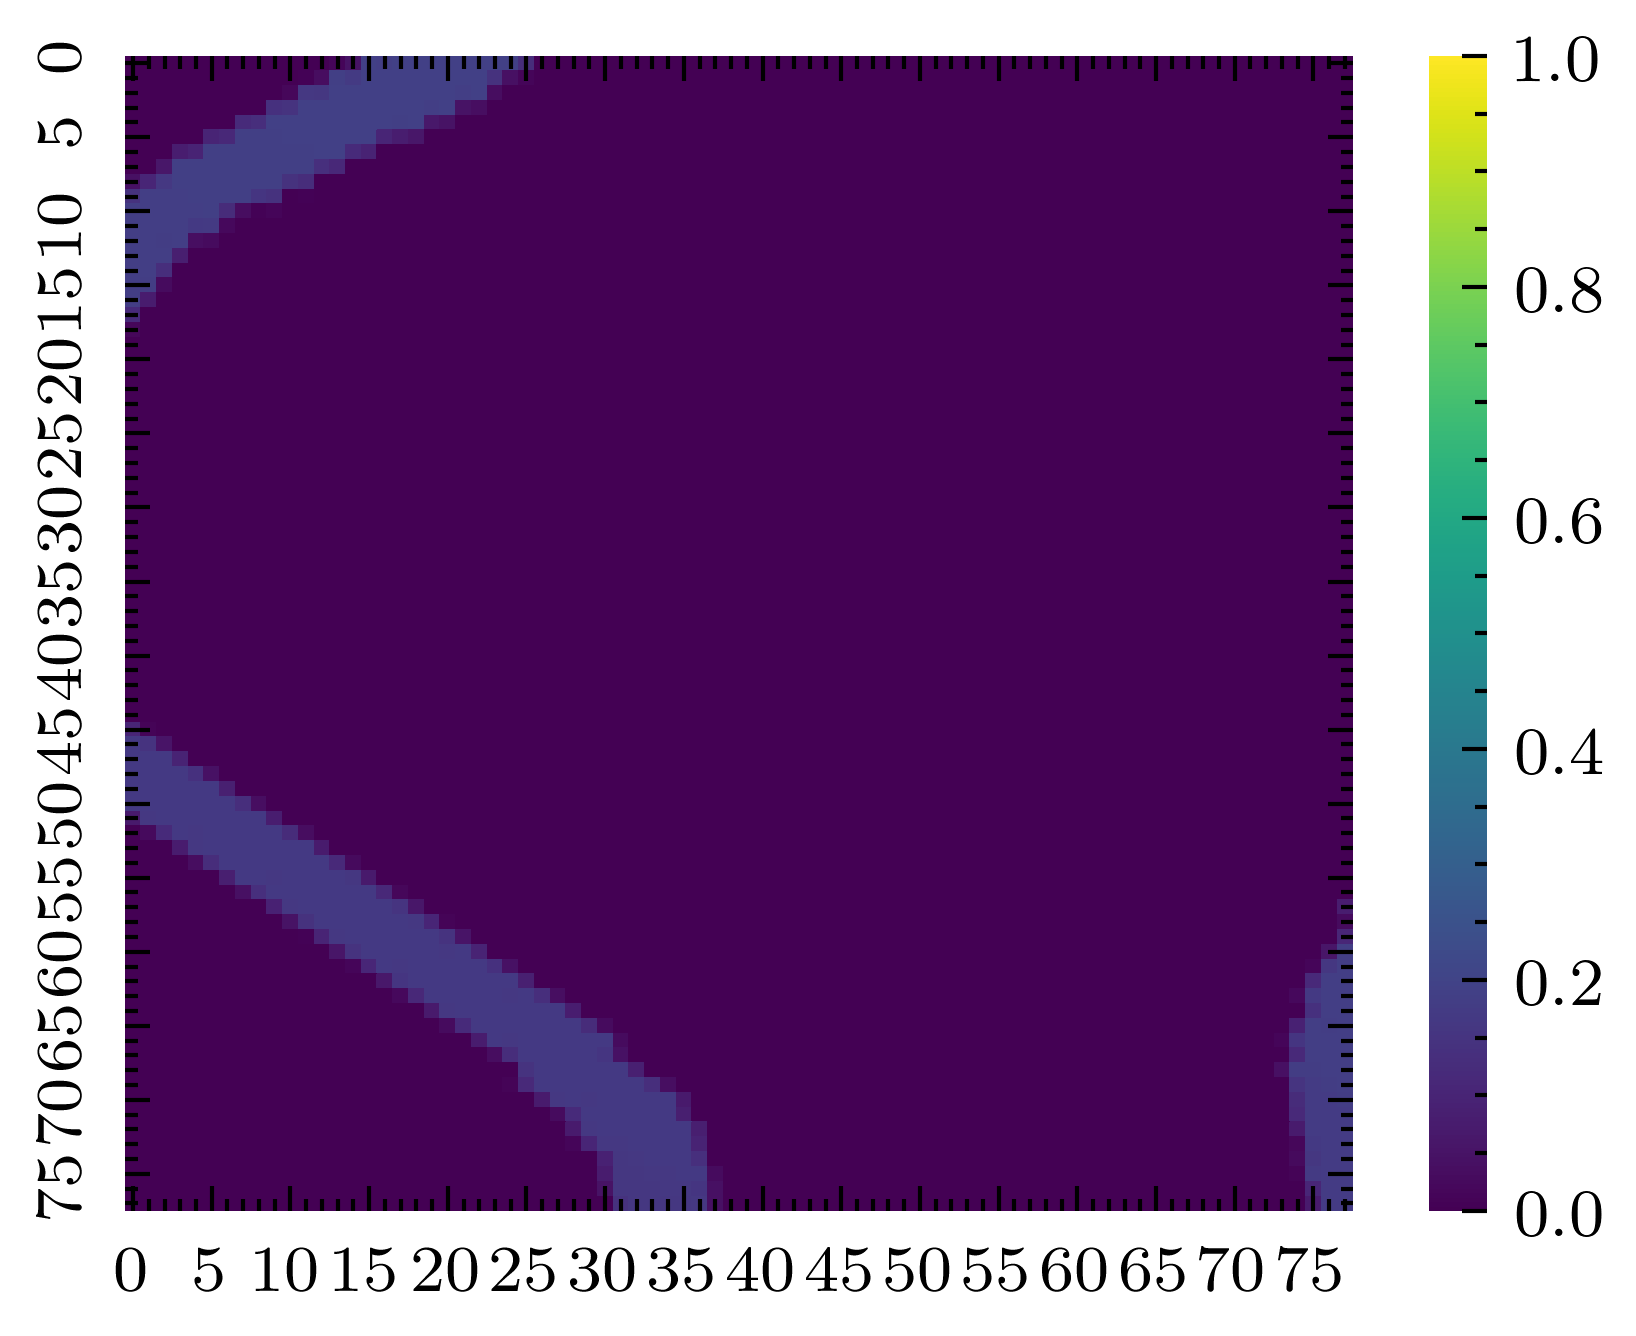
\includegraphics[width=\linewidth]{../img/bars1-example-patches/2d/0.png}
    \end{subfigure}
    \begin{subfigure}[b]{0.19\textwidth}
    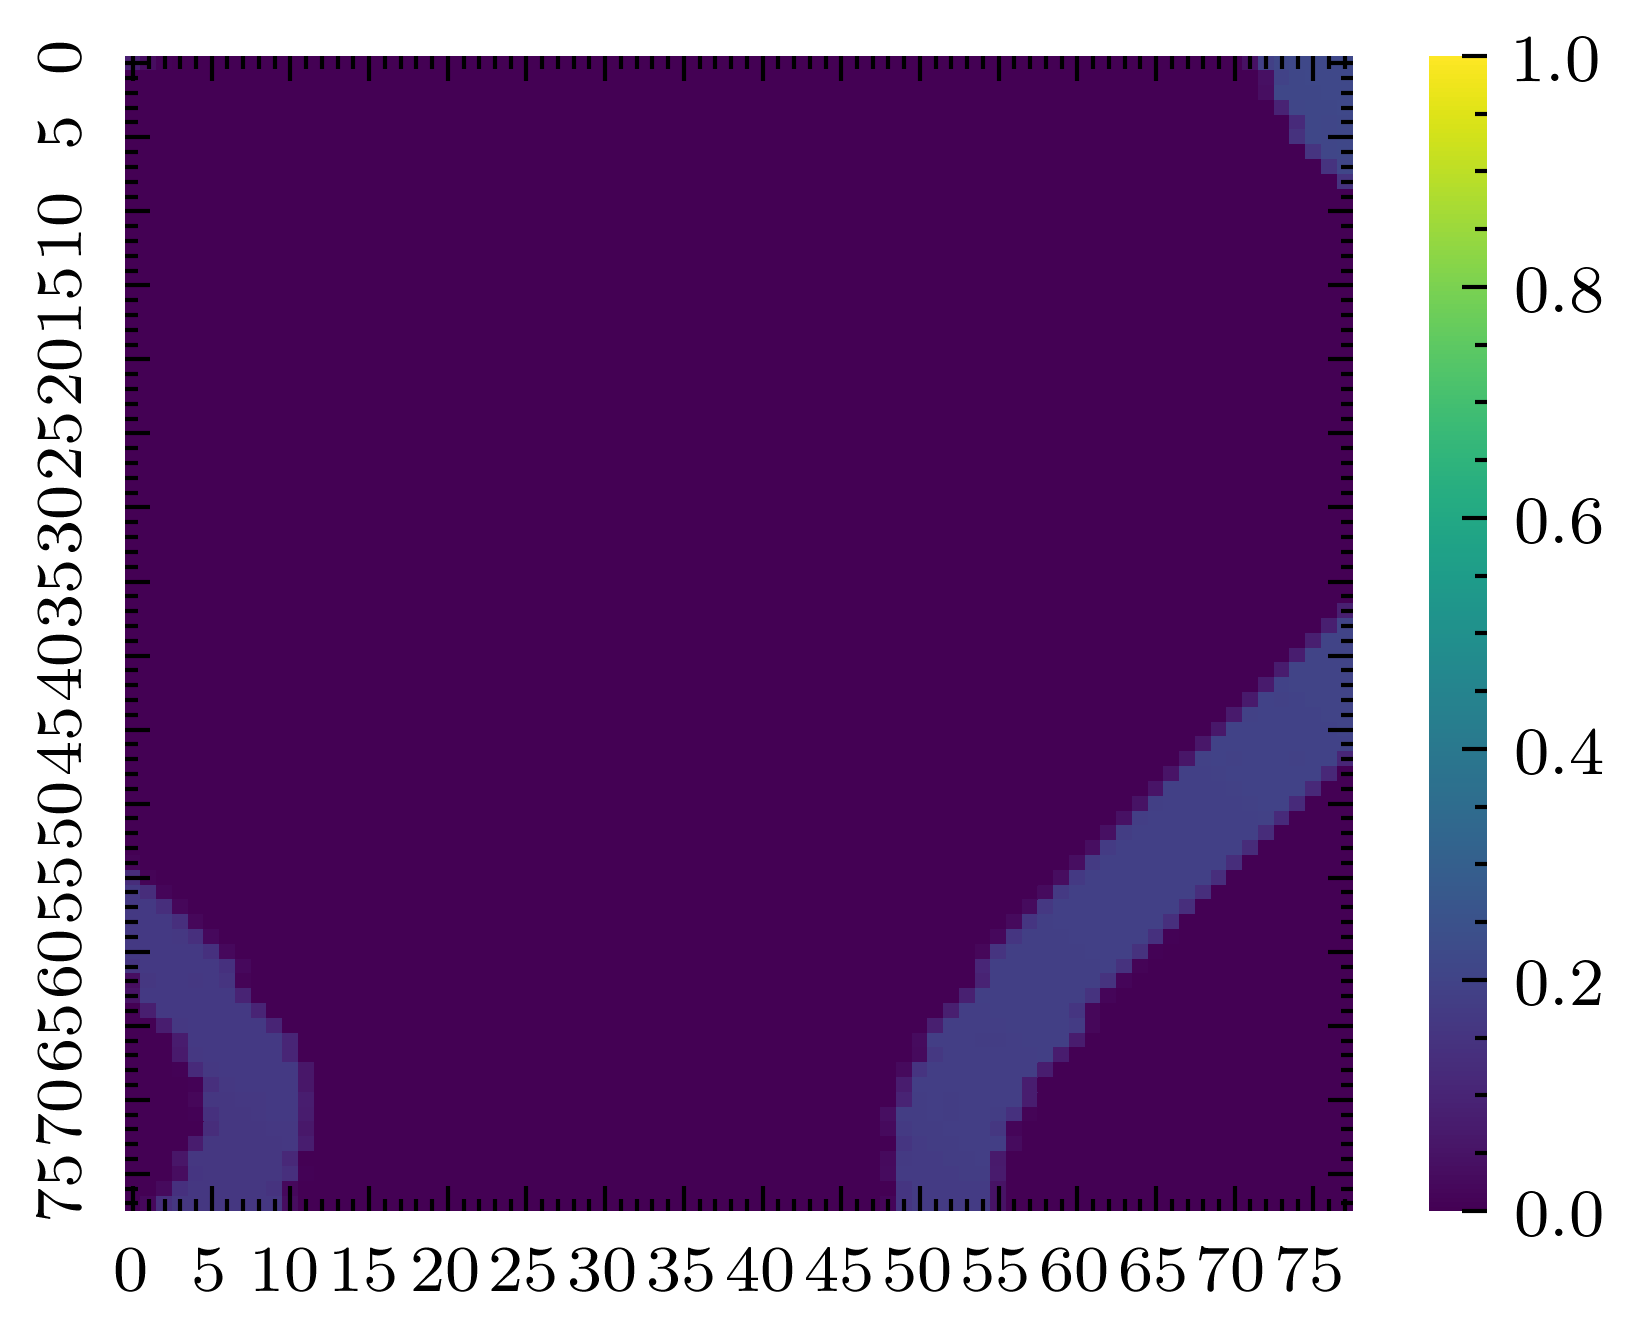
\includegraphics[width=\linewidth]{../img/bars1-example-patches/2d/2.png}    
    \end{subfigure}  
    \begin{subfigure}[b]{0.19\textwidth}
    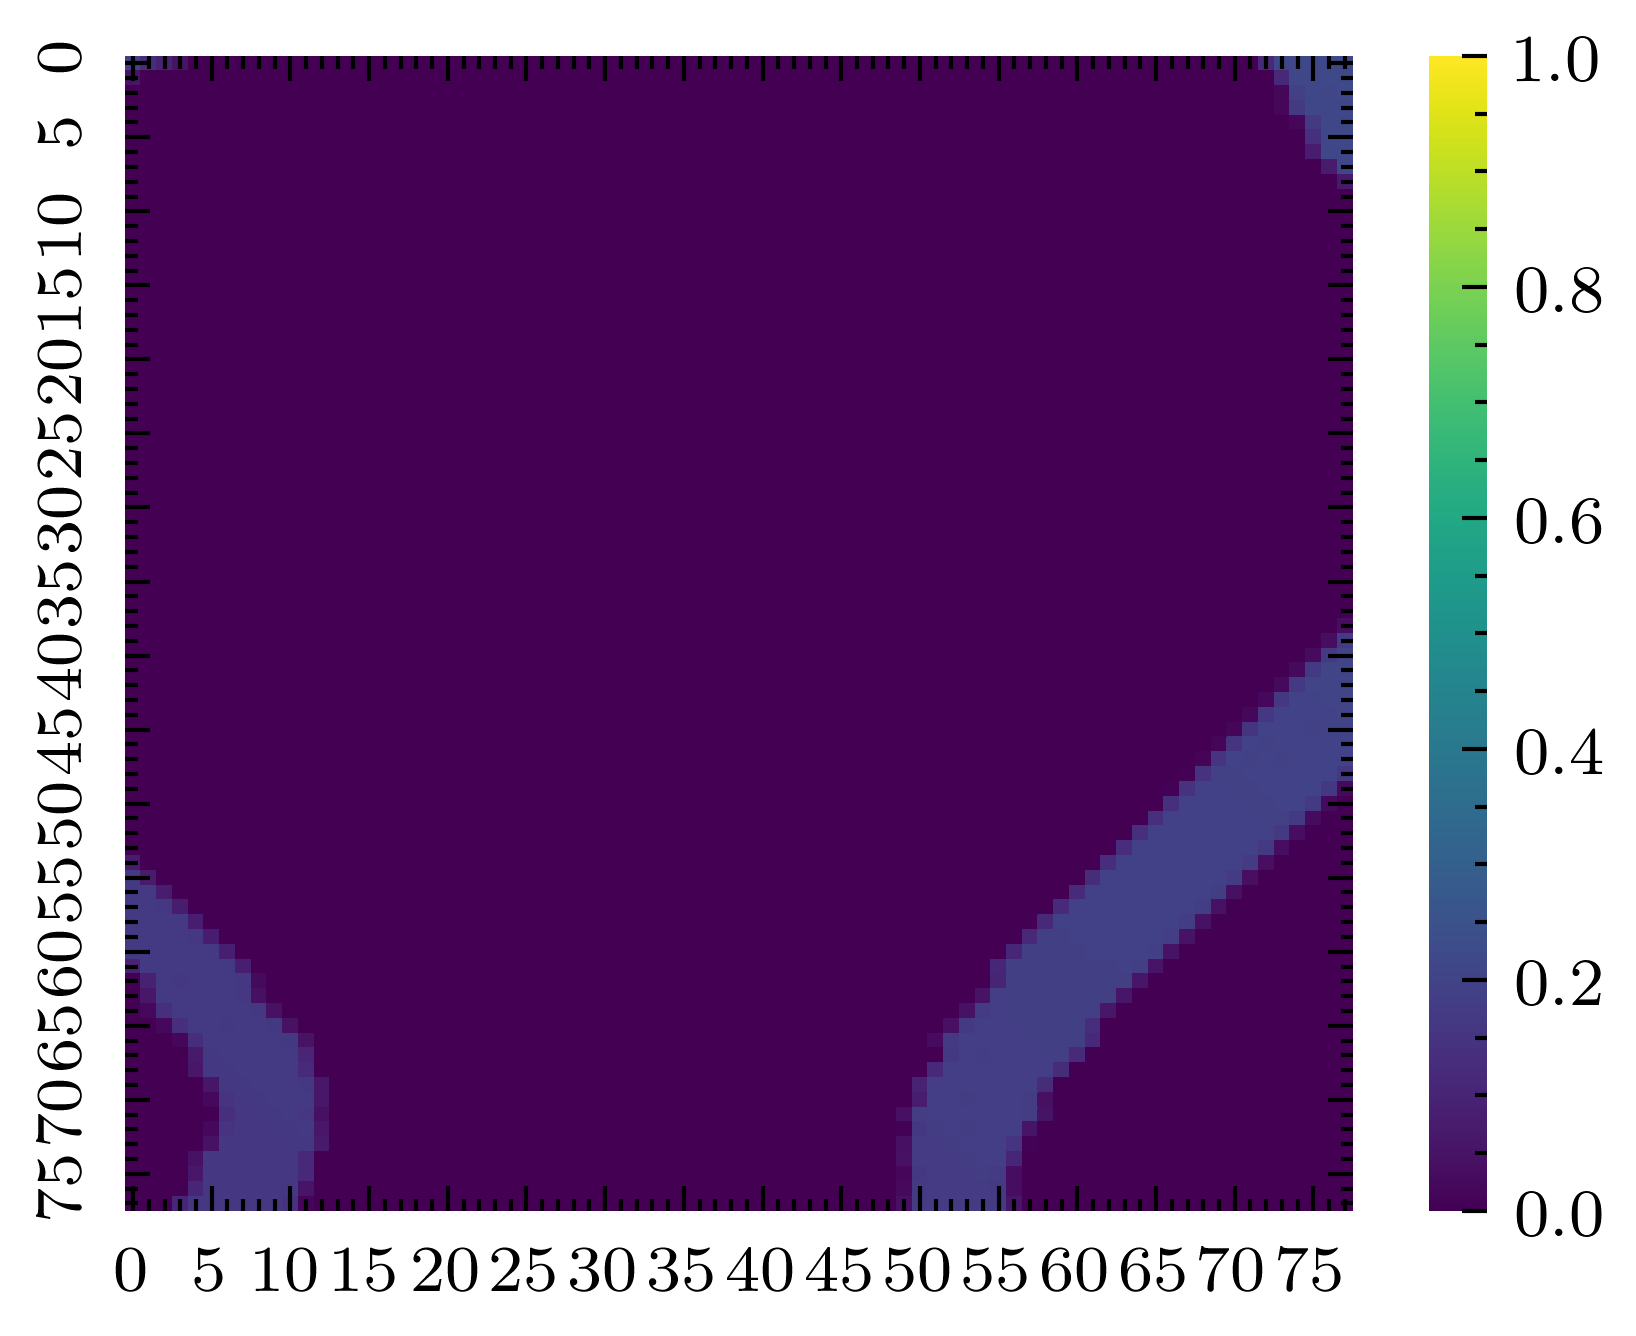
\includegraphics[width=\linewidth]{../img/bars1-example-patches/2d/4.png} 
    \end{subfigure}
    \begin{subfigure}[b]{0.19\textwidth}
    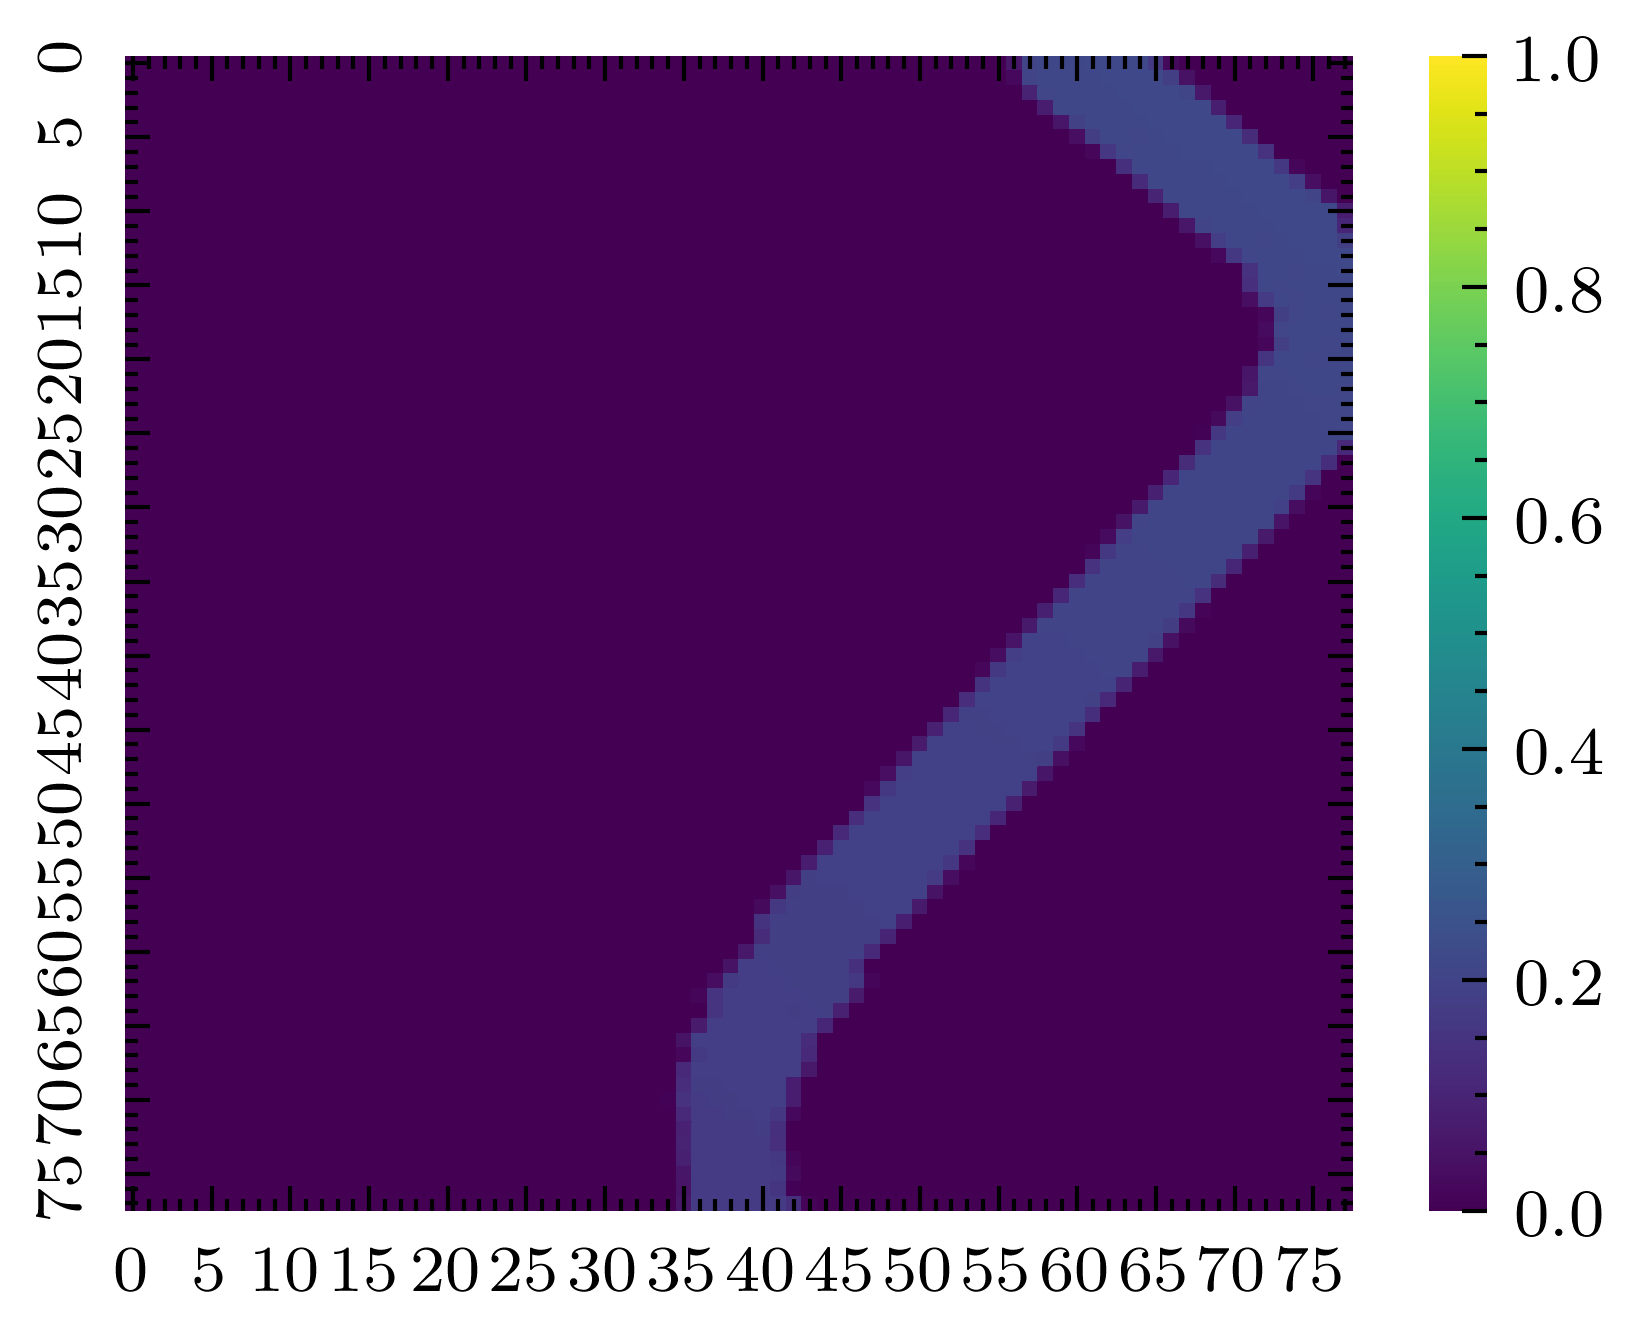
\includegraphics[width=\linewidth]{../img/bars1-example-patches/2d/7.png}    
    \end{subfigure}  
    \begin{subfigure}[b]{0.19\textwidth}
    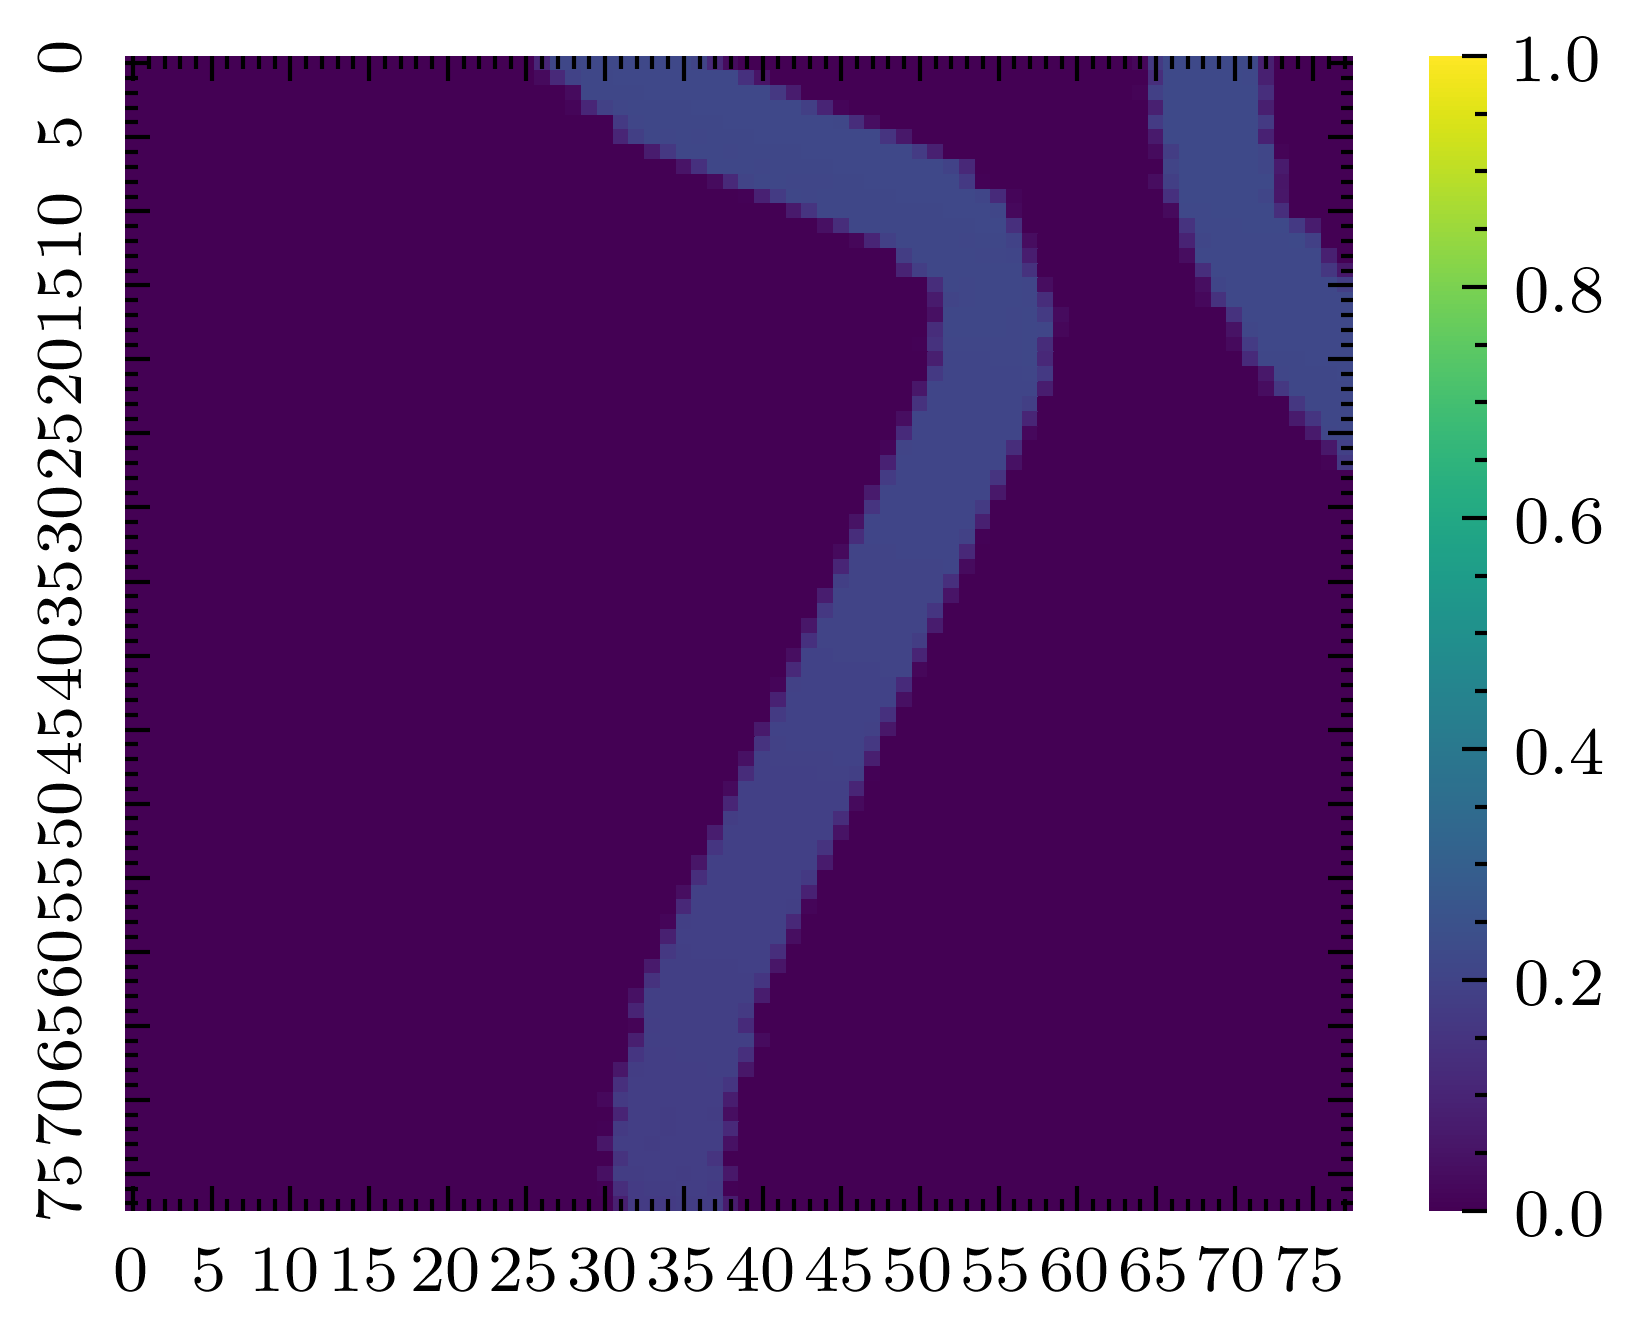
\includegraphics[width=\linewidth]{../img/bars1-example-patches/2d/14.png}    
    \end{subfigure}  
\caption{Cropped patches in 2D.}
\end{subfigure}  
\begin{subfigure}[b]{1\textwidth}
    \begin{subfigure}[b]{0.19\textwidth}
    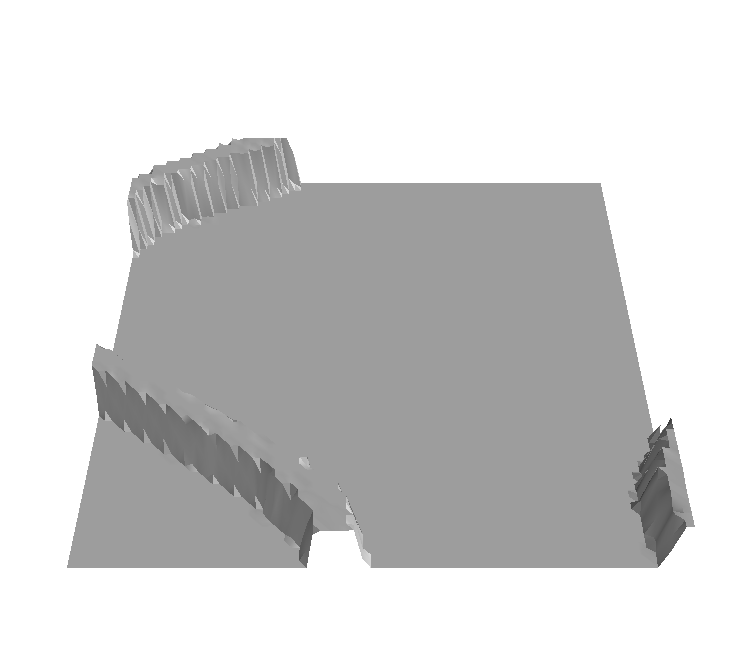
\includegraphics[width=\linewidth]{../img/bars1-example-patches/3d/0.png}
    \end{subfigure}
    \begin{subfigure}[b]{0.19\textwidth}
    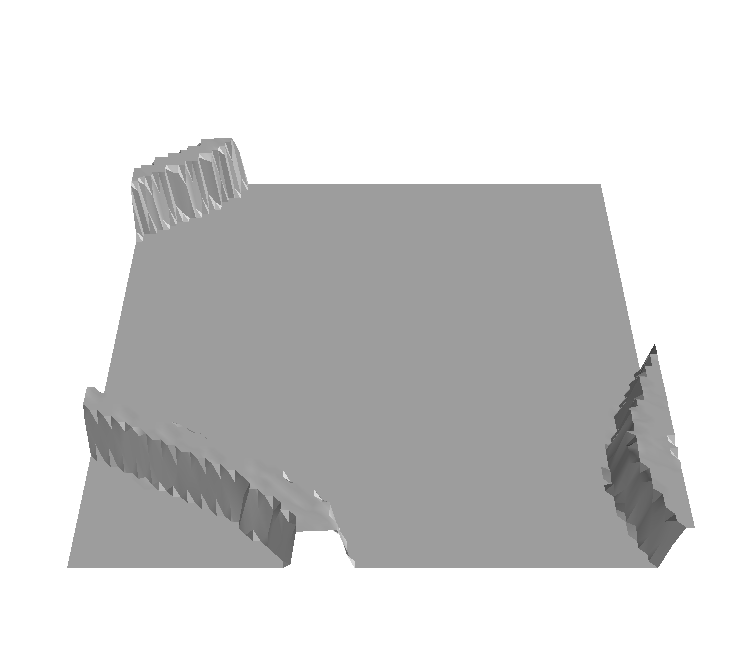
\includegraphics[width=\linewidth]{../img/bars1-example-patches/3d/2.png}    
    \end{subfigure}  
    \begin{subfigure}[b]{0.19\textwidth}
    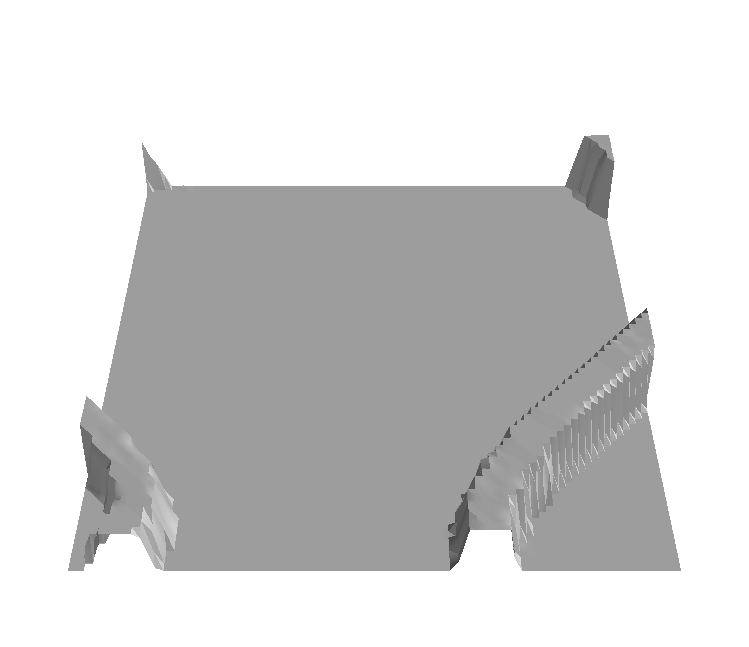
\includegraphics[width=\linewidth]{../img/bars1-example-patches/3d/4.png} 
    \end{subfigure}
    \begin{subfigure}[b]{0.19\textwidth}
    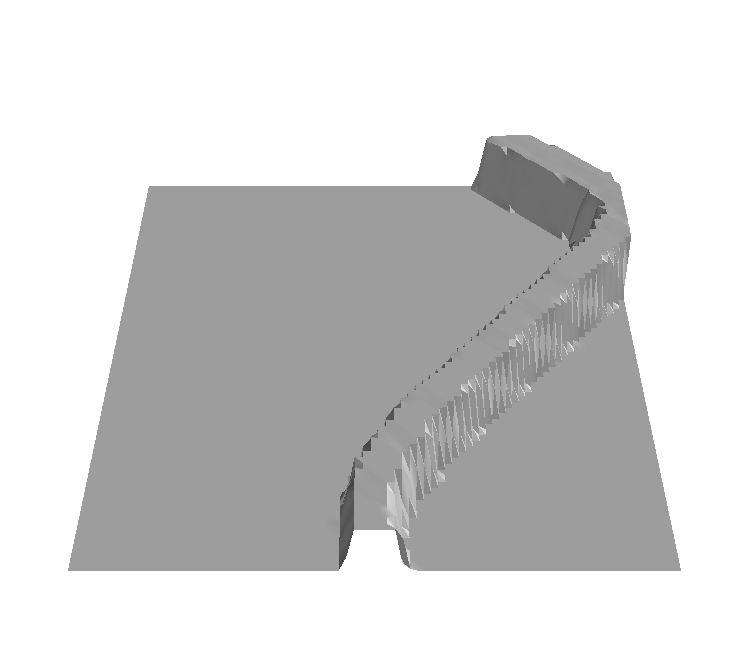
\includegraphics[width=\linewidth]{../img/bars1-example-patches/3d/7.png}    
    \end{subfigure}  
    \begin{subfigure}[b]{0.19\textwidth}
    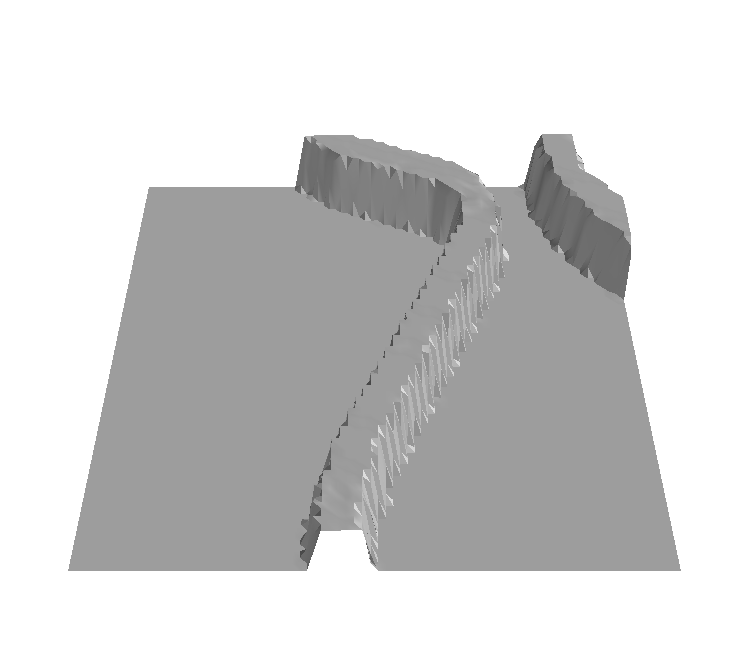
\includegraphics[width=\linewidth]{../img/bars1-example-patches/3d/14.png}    
    \end{subfigure}  
\caption{Cropped patches in 3D.}
\label{fig : patch-extraction}
\end{subfigure}
\caption{Example of a robot trajectory (a) extracted during training on a map with different walls. Robot's initial position is showed by its white siluette. Patches borders are label with greed if traversable and red if not and showed as 2D (b) and 3D(c) rendered images. The Robot traverse the patches from left to right.}
\end{figure}

This dataset is feed to a deep convolutional neural network. The network directly learns to extract and map features from raw data, in our case images, without needing to preprocess the inputs. We propose a model three times smaller than the original one with comparable performance. We evaluate all tested architecture using real world terrain, mostly obtained with flying drone and ground mapping software. 
We also investigate the model's learning by first visualizing the inputs that confuse the model. We adopted a technique that allows highlighting the regions in the input images that contribute the most to the prediction, in this way we can understand which part of the terrain was responsible for the wrong prediction. Lastly, we test the model's robustness by creating different patches with different characteristics and compare the prediction to the ground truth from the simulator. We show that the model is able to match the simulator's outputs in most scenarios but most important, we understand the network's limitations.

To summarize our contributions to the literature are the implementation of entire simulation based traversability framework that can be used with any mobile robot, a new small neural network architecture able to achieve high performances, different real-world evaluation and a model interpretability case study to understand strength and limitation of the trained model. 

\end{document}
